\chapter{State of the Art}\label{cap.estadodelarte}
\setlength{\parindent}{0pt}
\section{Neural Networks in Computer Vision}
Since the birth of Artificial Intelligence (AI) in 1956, the computer vision has followed a great rhythm of evolution. Taking the machines to equal humans in the resolution of some tasks, and in certain cases, to overcome them.
Artificial intelligence is defined in ~\cite{mccarthy2006proposal} as ``the subfield of Computer Science dedicated to developing programs that allow computers to present behaviors that can be characterized as intelligent". Machine learning (\textit{ML}) is defined in ~\cite{samuel2000some} as ``a field of Computer Science that gives computers the ability to learn without being explicitly programmed". Therefore, given this definition, the ML can be considered a subfield of the AI.\\
One of the most well known and currently growing ML subfields is called \textit{Deep Learning} ~\cite{deng2014deep}. This type of algorithm is intimately linked with the Artificial Neural Networks (\textit{ANN}) and in practice they are usually used in an equivalent way although they are not the same. One of the aspects to be highlighted in the Deep Learning algorithms is that it is no longer necessary to extract feature vectors for the input to the network. This is because these algorithms ``learn" how to represent the data in a hierarchical way. From these networks, the convolutional neural networks have a special interest to face the problem that this project presents. This type of networks are characterized by the use of a convolution operation in at least one of the layers of the network and their design for the processing of two-dimensional data such as images ~\cite{liu2015implementation}. In recent years, its evolution has been constant being able to overcome the results achieved by previous algorithms in tasks such as classification or detection of objects.\\

\subsection{Object classification and detection using neural networks}
Much of the progress made in recent years on the classification field of computer vision can be directly associated with a set of neural network architectures. The first big step forward came in 2012 when AlexNet ~\cite{krizhevsky2012imagenet} beats all the proposals of the state of the art at that time in the ImageNet challenge, ILSVRC. This competition of classification in images is a reference in the computer vision community. AlexNet obtained a test error rate of 15.3\% compared to the previous year's winner which was 26.2\%. This network, together with the VGG networks ~\cite{simonyan2014very}, follows the basic design archetype of convolutional networks: a series of convolution layers, followed by max-pooling and activation layers before the final classification layers \textit{fully-connected}. MobileNet is a simplified version of Xception ~\cite{chollet2016xception} for mobile applications that is currently behind the computer vision applications used on Google mobile devices.\\
The ResNet and Inception architectures, among others, are been used as blocks that serve as the basis for numerous subsequent works in computer vision and are briefly commented below:
\begin{itemize}
\item \textbf{Res-Net} ~\cite{he2016deep}: this network tries to solve the problem that seems to appear when adding layers to a network and that is that it generally behaves worse. For this reason, the authors propose that instead of trying to learn the hidden \textit{mapping} of the input \textit{x} to the function \textit{H(x)}, learn the difference between the two, that is, the residue (\textit{residual net}). For the calculation of H(x) they simply add the residue to the input and re-enter the next layer. This is a big change at the time as it solves the problem of the \textit{vanishing gradients} that the neural networks have suffered until the date. In addition, it allows to create much deeper networks, that is to say, with more layers, that allow better results.
\item \textbf{Inception} ~\cite{szegedy2015going}: this family of networks looks for wider networks, that is, with more intermediate operations between layers. The authors try to increase neural networks, in terms of operations, without an increase in computational cost. Introducing different parallel convolution operations the density of extracted information increases but also the computational costs. To solve the problem they use 1x1 convolutions to reduce dimensionality while performing different transformations in parallel. The resulting networks are simultaneously deep and wide.\\
The first version of Inception, known as GoogLeNet, was the winner of the 2014 ILSVRC. It was improved later with Inception v2 and v3. The last Inception v4 creates a hybrid with ResNet, known as Inception-ResNet ~\cite{szegedy2017inception}.
\end{itemize}
With the arrival of autonomous vehicles, intelligent video surveillance, face detection and numerous emerging applications, faster and more accurate detection systems are increasingly in demand. This includes not only recognizing and classifying each object in the image but also locating it with its corresponding text{bounding box}. This makes object detection significantly more complicated than traditional image classification. However, the most successful object detection algorithms today are extensions of image classification models.\\
The main object detection models are then introduced ~\cite{fu2017dssd}.  %cambiar: modify classification to remark difference between regionbased and singleshot
\begin{itemize}
\item \textbf{Faster R-CNN} ~\cite{ren2015faster}: is one of the current reference models and one of the last detectors known as  \textit{region-based} from Girshick \etal{}. This models basically work in the following way: they use some mechanism to extract regions from an image that are probably an object and then classify those proposed regions with a CNN. The father of this model is the R-CNN and it was the real driver of this type of techniques ~\cite{girshick2014rich}. In the proposed regions obtained through an algorithm called \textit{Selective Search} the characteristics are extracted through a CNN by region and then those regions are classified based on the characteristics. But its performance was slow.\\
This performance improves with Fast R-CNN ~\cite{girshick2015fast} for two main reasons. The first is that the CNN is applied over the whole image instead of over each region and then the regions are obtained from the last map of characteristics of the network. The second is due to the introduction of a Softmax layer that simplifies classification. Its mechanism was faster and easier to train than R-CNN but there was still a bottleneck in the generation of regions.\\
To solve it the RPN (\textit{Region Proposal Network}) is introduced and added to the Fast R-CNN it creates Faster R-CNN. The RPN returns proposed regions based on a \textit{score} that refers to the probability that the bounding box is an object, the \textit{objectness} (Figure \ref{fig:fasterrcnn}). And these regions are passed directly to the Fast R-CNN.\\
\begin{figure}[h!]
\begin{center}
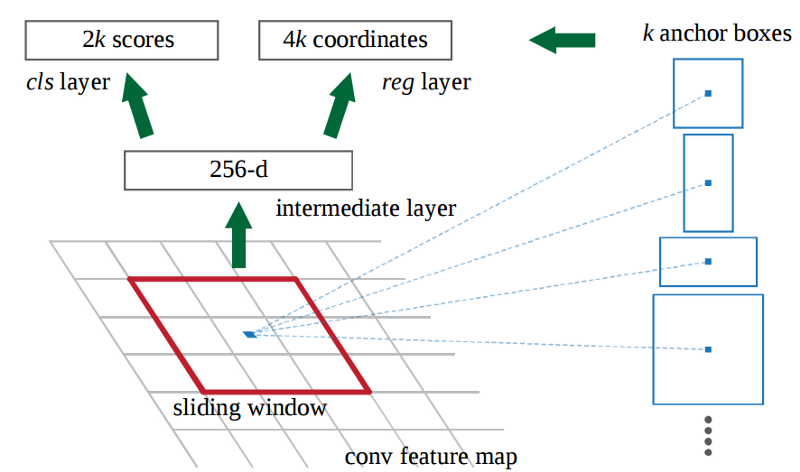
\includegraphics[scale=0.25]{faster_rcnn.png}
\caption{Region Proposal Network (RPN)}
\label{fig:fasterrcnn}
\end{center}
\end{figure}
\item \textbf{Overfeat} ~\cite{sermanet2013overfeat}: winner of the ILSVRC 2013 in location and detection of objects, this work showed that training a convolutional network to simultaneously classify, locate and detect objects in images can enhance the success both in classification, detection and location. Subsequently, it has been replaced by SSD and YOLO for tasks that require better detection in real time.
\item \textbf{R-FCN} ~\cite{dai2016r}: there are faster models than Faster R-CNN such as R-FCN, which tries to improve system speed by maximizing shared computing. %añadir algo mais
\item \textbf{SSD} ~\cite{liu2016ssd}: it provides great speed gains over Faster R-CNN by performing the phases of generating regions of interest and subsequent classification jointly (\textit{Single Shot MultiBox Detector}). As a result you get a lot of bounding boxes which most of them are not useful. By applying the techniques \textit{non-maximum suppression} and \textit{hard-negative mining} the final detections are achieved.
%explain nms and hardnegativemining %ampliar ssd xa que se usa
\item \textbf{YOLO} ~\cite{redmon2016yolo9000}: this model uses a different approach with respect to the above because it applies a single neural network to the entire image. This network divides the image into regions and predicts the bounding box and probabilities of each region. These are then weighted with the probabilities to obtain the definitive detections. This performs, as the authors indicate, a hundred times faster than Fast R-CNN, for example, maintaining a similar accuracy.\\ In YOLOv2, some improvements are introduced as FCN.
%ampliar con yolov2 e yolov3
\end{itemize}
In the following table obtained from ~\cite{redmon2016yolo9000} it can be seen how YOLO is almost on a par with methods like SSD or Faster R-CNN. On the other hand, it has a better balance between speed and accuracy since it manages to work in some cases at 91 FPS (\textit{frames per second}) when Faster R-CNN barely reaches 10 FPS (see Table 3 in ~\cite{redmon2016yolo9000}).
\begin{table}[h!]
\begin{center}
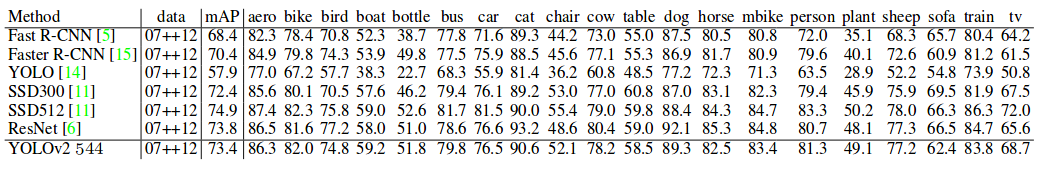
\includegraphics[scale=0.35]{yolo_results_pascal12.png}
\caption{Accuracy comparison in test phase in detection on PASCAL VOC 2012}
\end{center}
\end{table}
\subsection{Segmentation using neural networks}
La comunidad en visión artificial ha mejorado los resultados obtenidos en detección de objetos y segmentación semántica en un corto período de tiempo gracias, en gran parte, a poderosos sistemas de base como Faster R-CNN. En este proyecto se tratará de realizar segmentación de instancias, lo cual requiere de la correcta detección de todos los objetos en la imagen junto con la segmentación precisa de cada instancia. Así, cada píxel pertenece a alguna de las diferentes categorías sin diferenciar que se encuentre o no en un determinado objeto.\\ %reescribir
Driven by the effectiveness of the R-CNN family many of the methods proposed for instance segmentation are based on segment proposals where segmentation precedes object type recognition ~\cite{pinheiro2015learning}. This has proved to be slower and more inaccurate than if the prediction of object masks and class labels were done in parallel and separately. Li \etal{} propose a system known as FCIS (\textit{Fully Convolutional Instance Segmentation}) ~\cite{li2016fully} that tries to predict the output of a set of position-sensitive channels in a completely convolutional way. These channels perform the tasks of class, bounding box and masks calculations simultaneously which makes them faster. But it shows errors in instances that overlap creating spurious edges systematically (Figure \ref{fig:fcis_mask}).
Recently, Mask R-CNN ~\cite{he2017mask} arose to solve many of these problems and to situate itself as a state-of-the-art technique in segmentation of instances as can be seen in Figure \ref{fig:fcis_mask}. Por ello esta sección se va a centrar en esta técnica y sus resultados.\\ %revisar se hai algo novo neste tema e definir segmentacion semantica, de instancias etc
\begin{figure}[H]
\begin{center}
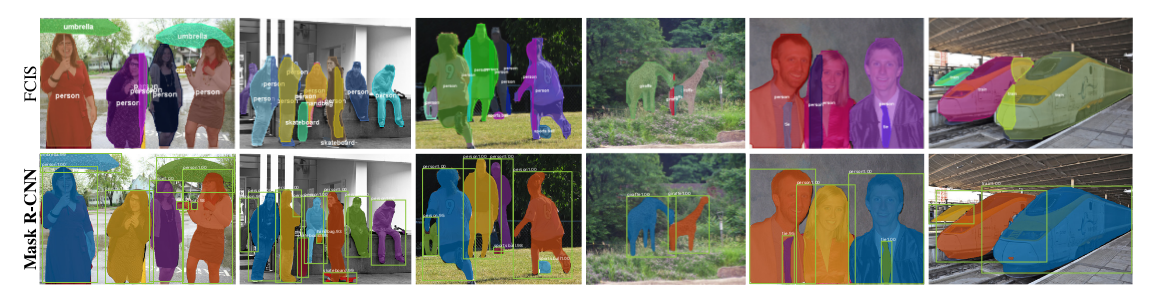
\includegraphics[scale=0.30]{fcis_vs_maskrcnn.png}
\caption{Results obtained by FCIS and Mask R-CNN in test images from COCO Dataset}
\label{fig:fcis_mask}
\end{center}
\end{figure}
Conceptually, Mask R-CNN adds a third stage to Faster R-CNN in which it obtains the mask of the object. The first stage of RPN coincides with that of Faster R-CNN while in the second stage it calculates, in parallel with the prediction of the class and the bounding box, a binary mask for each region of interest (\textit{RoI}). The generation of masks for each class is done without the classes competing with each other, which allows to separate the mask and class predictions from the object prediction. According to the authors, this proves to be the key to obtain good results in the final segmentation.\\ 
Another key factor in the proper functioning of this method is the correct alignment between the RoI and the extracted characteristics. This is usually done using \textit{RoIPool} in Fast R-CNN but introduces misalignments if the purpose is to segment rather than classify. This is why Mask R-CNN authors create \textit{RoIAlign}. To demonstrate the generality of the proposed method the authors introduce the mask prediction branch on several existing neural network architectures such as Faster R-CNN with ResNet as feature extractor, for example, and manage to surpass the winners of the 2015 and 2016 COCO Challenge segmentation, MNC ~\cite{dai2016instance} and FCIS ~\cite{li2016fully}. These experiments use COCO's standard metrics.\\
\begin{table}[h!]
\begin{center}
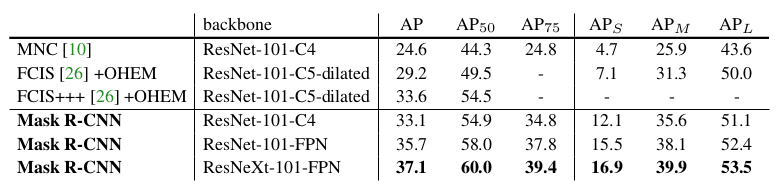
\includegraphics[scale=0.40]{mask_vs_mnc_fcis.png}
\caption{Results obtained from Mask R-CNN vs the previous works in segmentation on test images from COCO dataset}
\end{center}
\end{table}
As can be seen, all implementations of the Mask R-CNN model surpass the previous base models of the state of the art in instance segmentation.\\
Los autores también han realizado experimentos del rendimiento de esta técnica en el dataset Cityscapes (comentado en la sección 1.3). Para las categorías \textit{persona} y \textit{coche} este dataset presenta un gran número de instancias de diferentes clases solapadas, esto hace aún más complicada la correcta segmentación de instancias. Sin embargo, Mask R-CNN mejora los mejores métodos actuales en esta tarea y se convierte en método estado del arte. %necesario?
%------------------------------------------------------------------------
\section{Datasets in Computer Vision}
The datasets used when implementing or testing a certain system are key, since they influence the performance that the system can achieve. They also allow for a comparison of the solution found with respect to others that are part of the State of the Art in the task that is carried out, since they are usually associated with some type of competition. Therefore, it is necessary to correctly choose the dataset or datasets used in a computer vision problem. Here are some of the most well-known datasets used in many applications in the computer vision field:
\begin{itemize}
\item \textbf{COCO (Common Objects in Context)}\footnote {\href{http://cocodataset.org/#home}{COCO Dataset}}: it is a large scale dataset for detection and segmentation of objects mainly. It contains 80 categories of objects and 330000 images of which more than 200000 are labeled. It is a dataset widely used between the community and in congresses such as the ICCV (International Conference on Computer Vision).
\item \textbf{PASCAL VOC}\footnote {\href{http://host.robots.ox.ac.uk/pascal/VOC/}{PascalVOC Dataset}}: this dataset is linked with another challenge, the Pascal VOC Challenges. They ran this competition from 2005 to 2012. This project provides standardised image datasets for object class recognition, segmentation or action classification tasks.
\item \textbf{ImageNet}\footnote {\href{http://www.image-net.org/}{ImageNet Dataset}}: it consists of 14 million images approximately and an average of 500 images per category. It organizes the well-known ILSVRC competition (ImageNet Large Scale Visual Recognition Challenge) of location and detection of objects in images and videos. It is one of the reference datasets in this area.
\item \textbf{KITTI}\footnote {\href{http://www.cvlibs.net/datasets/kitti/}{KITTI Dataset}}: centered in the autonomous driving field, this vision benchmark suite introduces itself as a novel challenging real-world computer vision benchmark. The main areas of interest include 3D/2D object detection, 3D tracking or stereo vision. The type of objects for object detection available are focused in the ADAS field such as car, van, truck, pedestrian or cyclist.
\item \textbf{Cityscapes}\footnote {\href{https://www.cityscapes-dataset.com/}{Cityscapes Dataset}}: this dataset focuses on semantic segmentation in urban scenes. It contains 30 kinds of objects, 5000 images labeled with a \textit{fine} label (more precise) and 20000 labeled with a \textit{coarse} label in 50 different cities.
\item \textbf{OpenImages}\footnote {\href{https://storage.googleapis.com/openimages/web/index.html}{OpenImages Dataset}}: it is a dataset of about 9 million images. This makes it the "largest existing dataset with object location annotations". It also has a bigger number of classes than other challenges as the previously cited COCO and PASCAL VOC, exactly 600 object classes. It must be mentioned that the label distributions are usually skewed and with OpenImages it ocurres too. This means that there are many more objects of some kinds than others.
\end{itemize}
There are many other datasets such as those from research centers like INRIA, MIT or Caltech, for example, that contribute to the continuous improvement of the computer vision.
\section{Object tracking}
\subsection{Datasets}
Apart from these it is necessary to talk about the datasets that are focused on the core part of this work, i.e. \textit{the visual object tracking}. The visual object tracking is a fundamental task in computer vision which has importance in many applications such as surveillance, autonomous vehicle or video analysis. This task, the same way as others in the field needs datasets from which create and evaluate the algorithms. The datasets used are also commonly associated with competitions that allow the benchmarking of the developed algorithms. This benchmarks often provide the most objective measure of performance and, for this reason, they are important guides for research in the area of study.

The visual tracking datasets are going to be divided according to their tracking target, that is, if they are focused on the tracking of a single object (SOT) or on the tracking of multiple objects (MOT).
\begin{itemize}
\item \textbf{Multiple object tracking}
\begin{itemize}
\item \textbf{MOT} ~\cite{milan2016mot16}\\
This dataset arises from the need to provide a general and standardized way to create multi-object tracking algorithms, evaluate the results and present them. In the recent past, the computer vision community has promoted several benchmarks for the evaluation of numerous tasks such as object detection, optical flow or stereo estimation that have advanced the state of the art in these areas. However, not so much effort has been made in the standardization of the evaluation of multiple target tracking.\\
As many other datasets it is associated with a challenge, the \textit{MOTChallenge}. With this challenge they try to create a unified framework for the evaluation of multi-target tracking. The dataset provides a collection of datasets, some of them coming from datasets already in use and some from new challenging data. The given data are video sequences as always occurs when working in tracking tasks.\\
The first release of the dataset named \textit{MOT15} was focused on multiple people tracking, following the tendence of other datasets. The pedestrian tracking is by far the most studied case in the tracking context. In the next releases, more significant classes generally seen in urban scenarios were added like vehicles, bicycles or motorbikes. The challenge has had three editions: \textit{MOT15, MOT16, MOT17}. In each of them the sequences were more challenging than the edition before. This can include different camera viewpoints and positions, more challenging weather conditions (cloudy, night, sunny). For example, the mean crowd density in MOT16 is three times higher when compared to the first benchmark release (MOT15).
\begin{figure}[h!]
\begin{center}
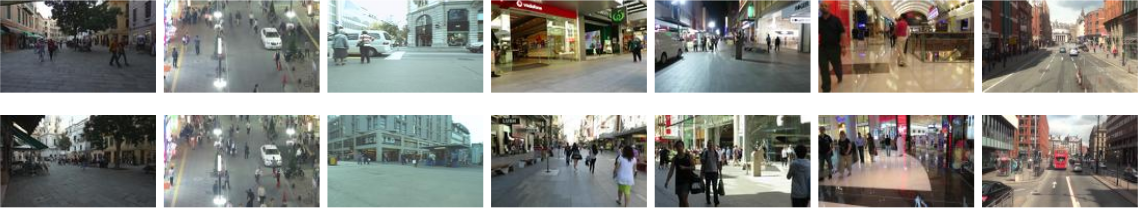
\includegraphics[scale=0.3]{mot16.png}
\caption{An overview of the MOT16 dataset. Top: Training sequences; bottom: test sequences ~\cite{milan2016mot16}}
\label{fig:mot}
\end{center}
\end{figure}
\item \textbf{ALOV}\footnote{{\href{http://alov300pp.joomlafree.it/dataset-resources.html}{ALOV Dataset}}}\\
The Amsterdam Library of Ordinary Videos for tracking is another well-known visual object tracking dataset in the field. It aims to cover as diverse circumstances as possible including illuminations, transparency, zoom or low contrast, for example. The dataset consists of 315 video sequences mainly obtained from YouTube with 64 different types of targets. The sequences are normally short with an average length of 9.2 seconds and the total number of frames is 89364 (in ALOV300).
\item \textbf{CAVIAR} \cite{dubuisson2016survey}\\
The CAVIAR project (Context Aware Vision using Image-based Active Recognition) from INRIA labs was dedicated to the development of algorithms that can describe and understand video scenes. The scenes were associated with surveillance scenarios where people performed some different activities related with the surveillance area. Those activities included \textit{walking}, \textit{browsing}, \textit{resting}, \textit{leaving bags behind} or \textit{two people fighting}. The annotations contain, apart from the bounding boxes locations, the head and feet positions, the body direction, among others. Refering to the tracking task, the challenging problems include occlusions, appearance/disappearance, appearance changing or similar object tracking, for example. In terms of data size, the first set contains 28 video sequences and the second set contains 44 video sequences (Figure \ref{fig:caviar}). It is a well-known dataset and is commonly used for development and testing of tracking algorithms.
\begin{figure}[h!]
\begin{center}
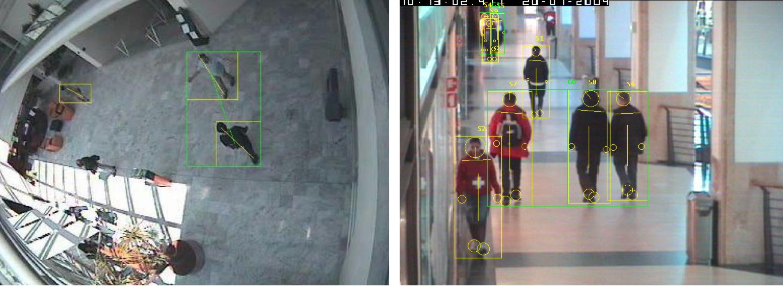
\includegraphics[scale=0.3]{caviar.png}
\caption{CAVIAR: From  left  to right, two frames (ground truth superposed) from sequences of datasets 1 (entrance lobby of INRIA Labs) and 2 (hallway of a shopping center) ~\cite{dubuisson2016survey}}
\label{fig:caviar}
\end{center}
\end{figure}
\item \textbf{BEHAVE} \cite{dubuisson2016survey}\\
Similarly to CAVIAR dataset, the BEHAVE Interactions Test Case Scenarios dataset contains various video sequences with different scenarios where people perform different interactions among which are \textit{walk together}, \textit{meet} or \textit{split} (Figure \ref{fig:behave}). The annotations include labels in case of interactions. Proposed for behavior analysis of interacing groups, this dataset was also used to validate visual for other purposes like the validation of visual tracking algorithms that consider occlusions or fast and varying motion of objects.
\begin{figure}[h!]
\begin{center}
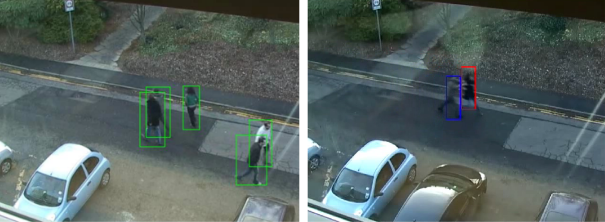
\includegraphics[scale=0.38]{behave.png}
\caption{BEHAVE: Two snapshots of sequences, with the ground truth bounding boxes of the objects to track \cite{dubuisson2016survey}}
\label{fig:behave}
\end{center}
\end{figure}
\item \textbf{PETS} \cite{dubuisson2016survey}\\
The International Workshop on Performance Evaluation of Tracking and Surveillance organizes a visual tracking competition with different objectives on every edition starting from 2000. In 2013\footnote {\href{http://www.cvg.reading.ac.uk/PETS2013/index.html}{PETS 2013}}, two of the objectives were the tracking and counting of people in crowds to estimate the density, and detecting events by crowd analysis. As BEHAVE or CAVIAR, PETS datasets are very popular among the computer vision community. The latest PETS edition took place in 2017\footnote {\href{http://openaccess.thecvf.com/content_cvpr_2017_workshops/w34/papers/Patino_PETS_2017_Dataset_CVPR_2017_paper.pdf}{PETS 2017}} and continued the evaluation theme of on-board surveillance systems for protection of mobile critical assets started in PETS 2016 \cite{patino2016pets}. On this edition, the dataset included sequences that adressed the protection of trucks (Figure \ref{fig:pets}) or vessels at sea, among others.
\begin{figure}[h!]
\begin{center}
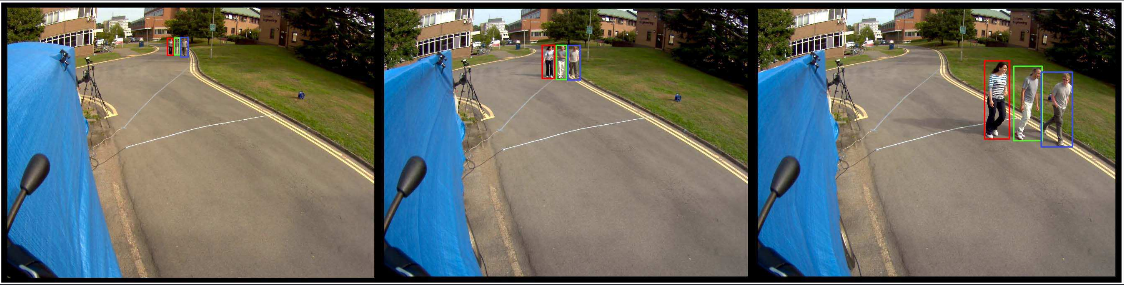
\includegraphics[scale=0.27]{pets2016.png}
\caption{PETS 2016: A group of people detected and tracked walking by the Truck \cite{patino2016pets}}
\label{fig:pets}
\end{center}
\end{figure}
\item \textbf{TrackingNet} \cite{muller2018trackingnet}\\
Most of the commented datasets are limited by its small size. Even more if they are going to be used by data-hungry trackers based on deep-learning. Currently, this trackers rely on object detection datasets due to the lack of dedicated large-scale tracking datasets. For this reason the authors created TrackingNet, the first large-scale dataset and benchmark for object tracking in the wild. TrackingNet provides a total of 30643 video segments with more than 14 million dense bounding box annotations (Figure \ref{fig:trackingnet}). The contributions of this work include different techniques to generate dense annotations from coarse ones and an extended baseline for state-of-the-art trackers benchmarked on TrackingNet. Referring to the latter, the authors affirm that pretraining deep models on this dataset can improve their performance on other datasets by increasing their metrics by up to 1.7\%.
\begin{figure}[h]
\begin{center}
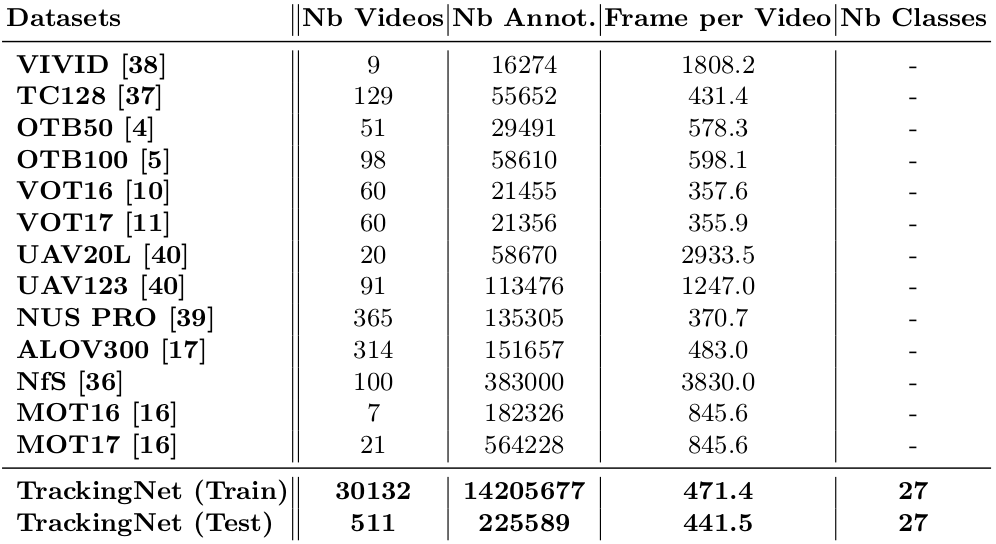
\includegraphics[scale=0.3]{trackingnet.png}
\caption{TrackingNet: Comparison of current datasets for object tracking \cite{muller2018trackingnet}}
\label{fig:trackingnet}
\end{center}
\end{figure}
\end{itemize}

\item \textbf{Single object tracking}
\begin{itemize}
\item \textbf{OTB} ~\cite{wu2013online}\\
As it was said before, for a comprehensive performance evaluation it is critical to collect a representative dataset. There exist several datasets for visual tracking in surveillance escenarios but often the target objects are humans or cars of small size with a static background. Also, some of the scenes are sometimes not annotated with bounding boxes which makes them not very useful for the comparison of tracking algorithms. To facilitate the evaluation task the authors built a tracking dataset with 50 fully annotated sequences in the first release \textit{OTB50}. Later, the dataset was extended with another 50 sequences (\textit{OTB100}).\\ Many factors can affect the tracking performance such as illumination variation or occlussion, for this reason the authors categorized the sequences with 11 attributes according to the occurrence of any of the selected factors (Figure \ref{fig:otb}).\\
\begin{figure}[h!]
\begin{center}
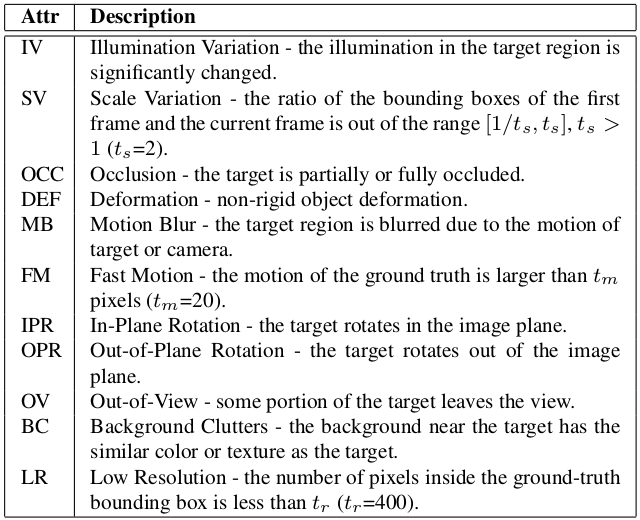
\includegraphics[scale=0.3]{otb_attributes.png}
\caption{OTB: List of the attributes annotated to test sequences ~\cite{wu2013online}}
\label{fig:otb}
\end{center}
\end{figure}
Apart from the data side, the authors also integrated most of the publicly available trackers at the time to create a code library with uniform input and output formats to facilitate large scale performance evaluation. Including TLD \cite{kalal2010pn}, MIL \cite{babenko2009visual} or CPF \cite{perez2002color} making a total of 29 tracking algorithms.
\item \textbf{VOT} \cite{kristan2017visual}\\
The Visual Object Tracking initiative was started in 2013 to address performance evaluation of short-term visual object trackers. The short-term tracking means that trackers are assumed to not be capable of performing successful re-detection after the target is lost and they are therefore reset after such event. In all the previous editions the challenge considers single-camera, single-target, model-free\footnote{The only training information provided is the bounding box in the first frame}, causal trackers\footnote{The tracker does not use any future frames, or frames prior to re-initialization, to infer the object position in the current frame}, applied to short-term tracking. The main goal of VOT is establishing datasets, evaluation measures and toolkits for visual object tracking (as many other initiatives). The successive editions were made in conjunction with Computer Vision Conferences like ICCV or ECCV. In 2015, a subchallenge focussed on tracking in thermal infrared (\textit{TIR}) was made due to the growing interest in this kind of imaging. The 7th Visual Object Tracking Challenge VOT2019 workshop will be held in conjunction with the ICCV2019. With respect to the previous edition in 2018, this challenge edition introduces the evaluation of trackers that use 4 channels (\textit{RGB-IR} and \textit{RGB-depth}).\\
Referring to the data itself, the VOT datasets try to pay more attention to the diversity of the data and the quality of the content and annotation with respect to the quantity. For example, some datasets assign a global attribute to the entire sequence when it is happenning in a fragment of it. VOT dataset tries to avoid the assumption that the quality of the data is correlated with its size. The VOT Challenge has focused on developing a methodology for automatic construction and annotation of moderately large datasets from a  large pool of sequences (Figure \ref{fig:vot}). For example, they use sequences from datasets such as the OTB dataset.
\begin{figure}[h!]
\begin{center}
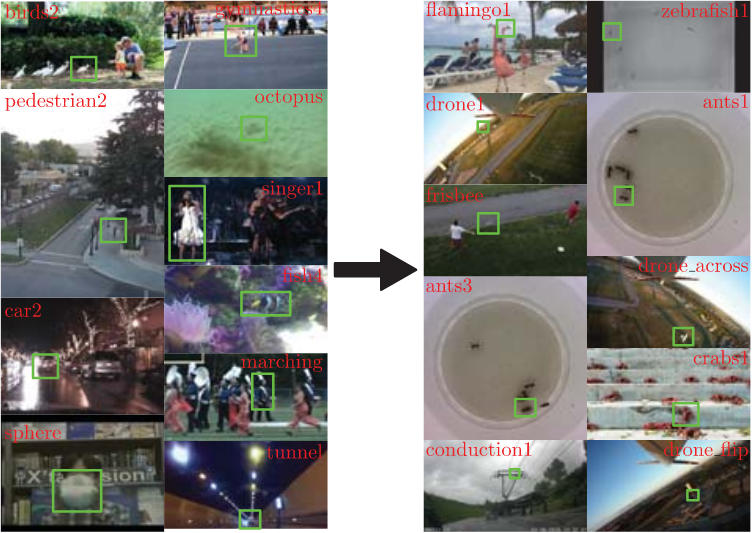
\includegraphics[scale=0.3]{vot.png}
\caption{VOT: Images from the VOT2016 sequences (left column) that were replaced by new sequences in VOT2017 (right column) ~\cite{kristan2017visual}}
\label{fig:vot}
\end{center}
\end{figure}
\item \textbf{Need for Speed} \cite{kiani2017need}\\
Visual object tracking algorithms have been usually evaluated at the canonical frame rate of 30 frames per second (\textit{FPS}) but consumer devices with cameras such as smartphones, tablets or drones are increasingly coming with higher frame rates. This can take time for the visual object track community to adapt to what \textit{real time} means in terms of how faster frame rates affect the choice of a tracking algorithm. The authors introduce Need for Speed (\textit{NfS}) as the first higher frame rate video dataset and benchmark for visual object tracking. The dataset consists of 100 videos captured with 240 FPS cameras from real world scenarios. The frames are annotated with bounding boxes and the sequences are manually labelled with nine visual attributes (occlusion, fast motion, etc.). The work also provide a ranking of many recent state-of-the-art trackers according to their tracking accuracy and real-time performance. One interesting conclusion the authors obtained is that at higher frame rates, simple trackers such as correlation filters outperform complex methods based on deep learning. This must be important when making the choice of a tracking algorithm in practical applications. It needs to be a tradeoff between the resources (available bandwidth, computation hardware, etc.) and the required application accuracy.
\end{itemize}
\end{itemize}
\subsection{Metrics}
%-------------------------------------------------------------------------
\subsection{Previous work on tracking}
Once the bases on which the project is based are seen, it is necessary to see what have been and are the works that form the State of the Art in the techniques that will be used to solve the problem that arises. Therefore, in this section we will talk about object tracking methods.\\ %cambiar
In the field of computer vision there is a wide variety of study areas, one of the most important is the so-called \textit{object tracking}. Its main objective is to estimate the state of the object (\textit{target}) over time in a series of sequences of images (\textit{frames}). This state can be defined by different characteristics such as shape, appearance, position or speed.\\
It is a difficult field since one or more circumstances can be given that must be solved by the algorithm. Among them are the management of variations in lighting and in the point of view of the object that can lead to changes in the appearance of the same. Likewise, the occlusions that occur when objects are mixed with other elements of the scene or the quality of the image itself may be a problem to consider in this area.\\
To confront these problems the following paradigms have been followed ~\cite{smeulders2014visual}:
\begin{itemize}
\item \textbf{Tracking using matching}: this group of algorithms makes a \textit {matching} between the representation of the model of the object created from the previous frame and the possible candidates in the next frame. The most outstanding methods are \textit{Normalized Cross-Correlation} ~\cite{briechle2001template}, \textit{Lucas-Kanade Tracker} ~\cite {baker2004lucas}, \textit{Kalman Appearance Tracker} ~\cite{nguyen2004fast} and \textit{Mean Shift Tracking} ~\cite{comaniciu2000real}.
\item \textbf{Tracking-by-detection}: a model is built to distinguish the object from the background ~\cite{nguyen2006robust}. Once you have the detection it is associated with the other detections. Currently, the community is turning to neural networks to compute detections.
\item \textbf{Tracking, learning and detection}: it is an extension of the previous group that includes a mechanism to update the model that is learned during execution. For example, you can use the results of a \textit{optical flow tracker} for this update ~\cite{kalal2010pn}. This ensures that the algorithm is invariant to changes in the object. 
\end{itemize}
Prior to the modern techniques to be discussed there are more classic ways of tracking objects that can be useful in problems that require real time when tracking, for example. One of the best known is \textit{feature tracking}. This technique uses characteristic points that can be found in the images and that allow to estimate the movement. These points must meet some requirements to be able to be characteristic of the image such as repeatability (the characteristic can be found in the images even if they have undergone some transformation), compatibility (each characteristic must be descriptive and easy to find) or efficiency (the representation of the information characteristic of the image must be done with as few characteristics as possible). Some of the characteristic points most commonly used are corners. They are characterized by gradients with higher values in them in two or more directions. These techniques include Harris ~\cite{harris1988combined} and Shi-Tomasi corner detectors ~\cite{shi1994good}.\\
There are tracking systems that take advantage of the speed of feature tracking and the accuracy of neural networks to create a hybrid tracking. In this type of tracking the detections are done each N frames using some type of neural network and the intermediate tracking is done through feature tracking.\\
With the arrival of neural networks this way of grouping the different tracking methods changes to adapt to them ~\cite{held2016learning}:
\begin{itemize}
\item \textbf{Tracking-by-detection}: they are designed to follow a certain class of object (\textit{model-based}) and to obtain a specific classifier. In the test phase the detections obtained with neural networks are linked using temporal information. They are limited to a single class of objects.
\item \textbf{Tracking, learning and detection}: they are characterized by being fully trained \textit{online}. A typical tracker example of this group samples zones close to the object and considers them "\textit{foreground}", the same happens with the distant zones that would be assigned to the "\textit{background}". With this you can build a classifier that differentiates them and estimate the new location of the object in the following frame ~\cite{babenko2009visual}. It has been tried to introduce neural networks in environments with online training but due to the slowness of the networks when training the results are slow in test phase.
\item \textbf{Siamese-based tracking}: this type of networks use \textit{patch-matching} techniques ~\cite{tao2016siamese}.   Multiple patch candidates from the new frame are received and the one with the highest \textit{matching score} with respect to the previous frame is chosen as the best candidate, that is, the most similar according to the matching function.
\item \textbf{Tracking as regression}: in this group, on the other hand, the network receives only two images and directly returns the location of the object ~\cite{held2016learning}.
\item \textbf{Tracking con RNN}: from the detection obtained this type of algorithms use \textit{Recurrent Neural Networks} to model the sequence of movement of objects thus improving the response to prolonged occlusions in time, for example ~\cite{sadeghian2017tracking}. They are the state of the art in tracking today. %revisar
\end{itemize}

